\documentclass{report}

\usepackage{mathtools, amssymb}
\usepackage{caption}
\usepackage[utf8]{inputenc}
\usepackage{subcaption}
\usepackage{graphicx}

\graphicspath{ {images/} }

\DeclarePairedDelimiter{\abs}{\lvert}{\rvert}
\DeclarePairedDelimiter{\norm}{\lVert}{\rVert}

\title{%
  Visual Odometry for Navigating in GPS Denied Environments\\[1in]
  \large Final Report Summary}

\date {December 2016}
\author{Alex Kreimer \\[1in] Department of Computer Science }

\begin{document}

\makeatletter
\begin{titlepage}
  \begin{center}
    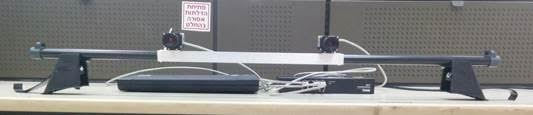
\includegraphics[width=0.7\linewidth]{title_cams}\\[4ex]
    {\huge \bfseries  \@title }\\[4ex] 
    {\LARGE  \@author}\\[50ex] 
  \end{center}
\end{titlepage}
\makeatother
\thispagestyle{empty}
\newpage

\section{Introduction}
In this work we revisit the problem of visual odometry. Visual
odometry is the process of estimating the motion of the camera by
examining the changes that the motion induces on the images made by
it. This work consists of two parts. In the first part we propose a
novel visual odometry algorithm.  In the second part we describe a
new data set.

The algorithm we propose exploits a scene structure typical for that
seen by a moving car and is suitable for use in either the stereo or
the monocular setting.  We recover the rotation and the translation
separately, thus dealing with two separate, smaller problems. The
rotation is estimated by means of the infinite homography. The
rotation estimation algorithm operates on distant image points using
the 3-D to partition them into the distant and the near-by ones. We
start with an initial estimate and then refine it using an iterative
procedure. After the rotation is compensated for, the translation is
found by means of the 1-point algorithm in the stereo setting and
epipole computation for pure translational motion in the monocular
setting.

We also created a new dataset that contains stereo video tracks
synchronized with the DGPS locations of the vehicle.  The dataset is
suitable for future visual odometry experiments and is interesting
because it has some challenging sequences (e.g. significant scene
occlusions by a moving vehicle , fast camera motion, rural scenery,
dusky sequences).

\section{Summary of Our Work}
In this work we present a novel algorithm for camera motion
estimation.  The novelty of the algorithm is in camera rotation
estimation procedure.  We rely on the fact that for scene points that
are infinitely far from the camera, the motion of the projected
(image) points may be described by an homography (the infinite
homography). For distant points this assumption is nearly true.  Our
algorithm starts by partitioning the scene points into two sets:
distant and near-by. Then, camera rotation is estimated from the
distant points and, subsequently, the translation is recovered from
the near-by points.

With respect to the classification of the visual odometry methods
given in the introduction, our work is local, feature based, stereo
odometry.  We do not use bundle adjustment, however the results of our
algorithm may be subsequently improved with some form of bundle
adjustment.

The outline of the our method:
\begin{enumerate}
\item Feature detection.  We use Harris corners.
\item Feature matching. The matching is done both across the stereo
  pair images as well as previous vs.\ current pair.  We enforce
  epipolar constraint, chierality and use circle heuristics similar
  to reject outliers.
\item Partition the scene points into two sets: distant and near-by.
\item Estimate the rotation of the camera from the distant points.
\item Estimate the translation of the camera from the near-by points.
\end{enumerate}

We choose the StereoScan as our baseline (our implementation of their
work).  The results in the show that on the KITTI dataset our rotation
estimation method outperforms the baseline.

We also build a dataset that contains a number of sequences that may
be used to benchmark visual odometry algorithms.  We install
synchronized stereo pair along a (D)GPS receiver on a car that travels
in an urban as well as rural areas.  Our goal is to cover some
challenging conditions that happen in day-to-day driving, e.g., field
of view occlusions, poor lighting conditions and low texture areas.

Note, that budget constraints led us to a simplified system that is
capable of producing 3DOF data (i.e., location only) being unable to
track vehicle orientation.

\end{document}

%%% Local Variables:
%%% mode: latex
%%% TeX-master: t
%%% End:
